\documentclass[10pt, conference, compsocconf]{IEEEtran}
\usepackage[T1]{fontenc}
\usepackage[utf8]{inputenc}
\usepackage[brazilian]{babel}
\usepackage{verbatim}
\usepackage{scalefnt}
\usepackage{xcolor}
\usepackage{ulem}
\usepackage{type1cm}
\usepackage{url}
\usepackage{subfigure}
\usepackage{courier}
\newcommand{\TODO}[1]{{\color{red}\textbf{\uwave{#1}}}}

\usepackage[pdftex]{graphicx}
\DeclareGraphicsExtensions{.png}

\title{Kalibro Metrics: a multi-repository and multi-language source
code analysis tool}

\author{
	\IEEEauthorblockN{Carlos Morais$^1$, Paulo Meirelles$^1$, Vin\'icius Daros$^1$, Fabio Kon$^1$}
	\IEEEauthorblockA{
		$^1$Department of Computer Science\\
		Institute of Mathematics and Statistics\\
		University of S\~ao Paulo, Brazil\\
		\{morais, paulormm, vkdaros, fabio.kon\}@ime.usp.br
	}
	
\and

	\IEEEauthorblockN{Carlos Santos Jr.$^1$$^,$$^2$}
	\IEEEauthorblockA{
		$^2$Horizon Institute\\
		University of Nottingham, United Kingdom\\
		carlos.denner@nottingham.ac.uk
	}

}

%-------------------------------------------------------------------------------
\begin{document}
\normalem
\def\UrlFont{\tt\footnotesize}
\maketitle

\begin{abstract}
Source code metrics are not new, but they have not yet been fully explored in
software development. For example, most metrics do not have known
thresholds to guide their use by non-experts.
%
Most metrics tools show isolated numeric values, which are not easy to
understand because the interpretation of these values depends on the
implementation context.
%
Kalibro Metrics goal is to improve the readability of source code metrics. It
allows a source code metric user to create a configuration of thresholds
associated with qualitative evaluation, including comments and recommendations.
%
Using these configurations, Kalibro shows metric results in a friendly way,
helping software engineers to spot design flaws to refactor, project managers
to control source code quality, and software adopters and researchers to compare
specific source code characteristics across free software projects.
%
These configurations are shared among its users via the Kalibro Web Service and
a source code tracking network to enhance metric results interpretation.

\end{abstract}
\vspace{1\baselineskip}

\begin{keywords}
Software metrics, source code analysis, thresholds configuration,
Web Service integration, source code tracking network, Free Software.
\end{keywords}





\IEEEpeerreviewmaketitle

%-------------------------------------------------------------------------------

\section{Introduction}
\label{introduction}




\section{Projeto}
\label{sec:projeto}


O Portal do Software Público Brasileiro (SPB), inaugurado em 2007, na prática, é um sistema
web que se consolidou como um ambiente de compartilhamento de projetos de software.
Oferece um espaço (comunidade) para cada software. A comunidade é composta por fórum,
notícias, chat, armazenamento de arquivos, downloads, wiki, lista de prestadores de
serviços, usuários, coordenadores, entre outros recursos. Teve um crescimento expressivo
contando, hoje, com mais de 60 comunidades de desenvolvimento e mais de 200.000 usuários
cadastrados. O SPB abrange também o 4CMBr, que é um grupo de interesse voltado para
soluções de tecnologia para municípios, o 5CQualiBr, que é um grupo que trabalha para
evoluir a qualidade do SPB, o 4CTecBr, que é um portal destinado a
colaboração no desenvolvimento de Tecnologias Livres, o Mercado Público Virtual, que é um
grupo de empresas e pessoas que prestam serviços nos softwares ofertados no Portal, e o Ava- 
liaSPB, que avalia a entrada dos softwares candidatos à software público. O ambiente do 
SPB não proporciona a integração com ambientes colaborativos externos, especialmente com
redes sociais. A plataforma escolhida na ocasião da criação foi o framework OpenACS, que
continua sendo utilizada na versão atual.
%
A evolução do SPB foi comprometida desde 2009, quando framework OpenACS foi 
descontinuado. Com isso, não tendo versões lançadas a partir daquele ano. Por isso, hoje,
é necessária a evolução para novas tecnologias que tenham maior suporte das comunidades
de desenvolvimento, que utilize linguagens de programação com maior rapidez de aprendizagem e
de desenvolvimento e que permita a integração com ambientes colaborativos externos, em especial, as
redes sociais. Além disso, é preciso realizar a manutenção evolutiva das funcionalidades
existentes e também o desenvolvimento de novas funcionalidades para o Portal do SPB.
%
Um dos passos para a concretização de uma nova geração do Portal SPB é a integração de
novas tecnologias, desde uma plataforma colaborativa até sistemas de controle de versão e de
monitoramento da qualidade do código fonte, gerenciadas e apresentadas em uma plataforma
integrada no back-end \footnote{O front-end é responsável por coletar a entrada em várias formas do
usuário e processá-la para adequá-la a uma especificação em que o back-end possa utilizar. O front-end é uma espécie de interface entre o usuário e o back-end.} 
e, em especial, no front-end \footnotemark[2] para que os usuários e as comunidades
tenham um conjunto de recursos para encontrarem os projetos, bem como colaborarem em torno 
de um sofware público.
%
Mesmo com as limitações citadas, o Portal do Software Público Brasileiro teve em 2013 
mais de 600 mil visitantes únicos, com mais de 1 milhão de visitas/acessos, gerando mais
de 16 milhões de visitadas nas páginas, com um total de mais de 49 milhões de hits \footnote{O número de vezes que os visitantes visualizaram uma determinada página no site.} no
Portal SPB. Avaliando apenas as comunidades dos projetos I3Geo, CAU, CACIC e Geplanes,
houve mais de 15 mil downloads e 4 mil mensagens nos fóruns. Essa amostra
ilustra bem o potencial do Software Público Brasileiro, bem como as expectativas de seus
usuários e colaboradores para a evolução do Portal e do modelo em si.

\section{Arquitetura e tecnologias propostas}
\label{sec:arquitetura}

O sistema que irá atender a evolução e reformulação do Portal do Software Público Brasileiro é composto por diversos módulos, os quais irão comunicar-se entre si de forma organizada e integrada para suprir as necessidades do projeto.
%

\begin{figure}[htpb]
  \begin{center}
    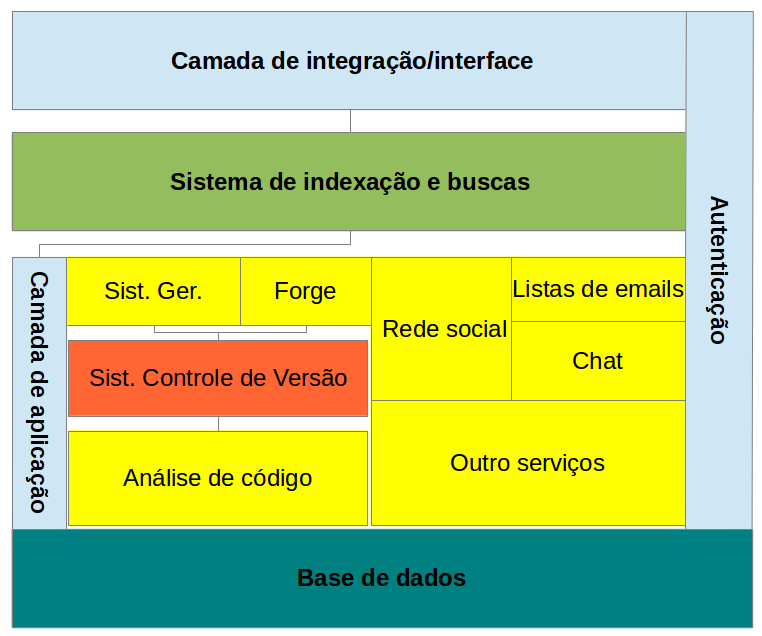
\includegraphics[width=.37\textwidth]{images/visao_arq.png}
  \end{center}
  \caption{Proposta de arquitetura do Novo Portal do Software Público}
  \label{fig:core_concurrent}
\end{figure}

No início do projeto realizamos estudos de possíveis ferramentas que pudessem ser utilizadas para atender as necessidades do projeto, chegando então na lista apresentada abaixo.
Na análise realizada chegamos ao entendimento que utilizar elementos já oferecidos por softwares livres existentes seria o ideal, pois eles já atendem às nossas necessidades, evitando o retrabalho e customizando os elementos necessários.   

As ferramentas que serão utilizadas para suprir essas necessidades serão:


\begin{itemize}
\scalefont{0.95}

\item Para lista de e-mail estamos utilizando o Mailman na versão 2, que é um software gratuito para gerenciamento de discussão eletrônica de e-mail e listas {\it e- newsletter};

\item Para Chat estamos utilizando Punjab BOSH (XMPP), que é uma interface HTTP cliente jabber. É um gerenciador de conexão BOSH que permite conexões de clientes persistentes para um servidor XMPP (protocolo de comunicação para mensagens orientadas a {\it middleware} baseado em XML);

\item Para Plataforma de Buscas estamos utilizando Apache Solr, que é uma plataforma de busca open source da Apache Lucene escrita em Java;

\item Para rede social estamos utilizando o Noosfero que é uma plataforma web livre para criação de redes sociais com blog, e-Portifólios, CMS, RSS, discussão temática, agenda de eventos, galeria de imagens, chat, entre outros. Ele foi desenvolvido pela Cooperativa de Tecnologias Livres – Colivre 3 em 2007, sob a licença AGPL v.3, com a proposta de permitir ao usuário criar sua própria rede social personalizada, livre e autônoma;

\item Para Forge para SVN estamos utilizando o Trac, que é uma ferramenta open source para controle de mudanças em projetos de desenvolvimento;

\item Para sistemas de controle de versão estamos utilizando SVN e Git, que são ferramentas open-source para controle de mudanças em projetos de desenvolvimento;

\item Para Forge para Git estamos utilizando o GitLab, que é um software livre de colaboração de código online que utiliza a ferramenta de gerência de código fonte Git;

\item Para sistema de gerenciamento estamos utilizando o Redmine, que é uma aplicação web de gerenciamento de projetos que disponibiliza diversas ferramentas para auxiliar a gestão e manutenção de um projeto;

\item Para suporte a Single Sign On estamos utilizando o Mozilla Persona, que foi desenvolvido pela Mozilla e permite o suporte a {\it single sign on};

\item Para Sistema de Integração contínua estamos utilizando o Jenkins, que é uma aplicação web de integração contínua de construção de projetos.
\scalefont{1}
\end{itemize}


Para integrar todas estas ferramentas estamos utilizando o Colab, que é uma plataforma de integração de ferramentas. Nele, são também integradas as interfaces das ferramentas para que, ao navegar, o usuário tenha a sensação de estar navegando em uma única ferramenta.



\section{Metodologia de Desenvolvimento}
\label{sec:metodologia}

A Engenharia de Software tem evoluído suas práticas e metodologias em busca de padrões que regem o desenvolvimento de software de qualidade dentro dos escopos, custos e prazos desejados. O modelo dito tradicional tem como característica um conjunto grande e detalhado de documentação que deve, supostamente, ser utilizada ao longo de todo o ciclo de desenvolvimento. Entretanto, percebendo que os objetivos principais do desenvolvimento de software não estavam sendo alcançados, alguns líderes da indústria e academia começaram a adotar métodos mais simples de trabalho que apresentaram melhores resultados em projetos de software. Em 2001, líderes que estavam desenvolvendo projetos fora dos padrões industriais se reuniram para trocar experiências e trabalhos. Este grupo se tornou a Aliança de Desenvolvimento Ágil e escreveram o Manisfesto Ágil que apresenta os princípios e valores que o grupo considera ser determinante para o desenvolvimento de software. Neste sentido, os métodos de desenvolvimento ágeis de software são métodos que implementam os seguintes valores:

\begin{itemize}

\item Indivíduos e interações acima de processos e ferramentas; 

\item Software operante acima de documentações grandes e completas; 

\item Colaboração do cliente acima de negociações contratuais; 

\item Responder à mudanças acima de seguir a um planejamento.

\end{itemize}

Esse conjunto de valores não descartam a importância dos elementos citados à direita das sen- 
tenças, mas evidenciam que estes são menos importantes diante dos primeiros elementos citados. 
Em outras palavras, apesar da documentação ser importante, o foco principal deve estar na entrega 
de software de valor para o cliente e na interação e a consequente comunicação entre as pessoas. 
Além disso, os métodos ágeis exaltam a simplicidade, feedback contínuo e adaptação à mudanças 
que podem ser obitidos a partir de comunicação face à face, qualidade de código e entrega contínua 
de software. 

Dada a oportunidade de adoção de métodos ágeis no desenvolvimento do presente trabalho, a 
metodologia utilizada é baseada em uma combinação das metodologias Scrum e Extreme Programming. Destacam que XP e Scrum complementam um ao outro bem, com o XP provendo suporte para aspectos mais técnicos enquanto o Scrum provê práticas e técnicas para gerenciamento, planejamento e acompanhamento. Assim,com base nas experiências destacadas em [Schwaber and Beedle, 2001] e 21 [Fitzgerald et al., 2006], na motivação de adoção de métodos ágeis no desenvolvimento de software moderno, serão apresentadas os métodos XP e Scrum, suas principais características e práticas que serão utilizadas no desenvolvimento do presente projeto.


\section{Escolha da equipe}
\label{sec:equipe}

	A equipe é formada, majoritariamente, por alunos de graduação do curso de Engenharia de Software da Universidade de Brasília, conta ainda com dois ex-alunos formados, alunos de mestrado, que trabalham exclusivamente com o design, e professores orientadores. 
	
	Devido a esta formação, a equipe não consegue estar sempre trabalhando fisicamente junta, pois cada membro da equipe possui horários particulares de aula e, com isso, o horário dedicado a contribuição do projeto pelos mesmos depende do horário dessas aulas. Dessa forma, não conseguimos utilizar integralmente as práticas das metodologias ágeis.
	
	A equipe do projeto está dividida em duas equipes: equipe Noosfero e equipe Colab, a qual também atua na integração com outras ferramentas. A equipe do Noosfero está desenvolvendo um plugin com novas funcionalidades para o Portal do Software Público. A equipe do Colab está, no momento, trabalhando com configurações das ferramentas, pois está sendo realizada a integração do Redmine e do Gitlab com o Colab, o que exige maiores esforços de infra-estrutura.
	
	Para manter o controle das atividades do projeto e evitar os ruídos de comunicação temos uma lista de e-mail com todos os integrantes do projeto, onde foi criado o hábito de enviarmos um e-mail ao final do dia com as atividades que desenvolvemos, e a ferramenta de gerenciamento Redmine, onde são escritas as histórias de usuários, as histórias técnicas e suas respectivas tarefas. Realizamos ainda um stand-up em todos os dias de trabalho,em que todos estão ou no laboratório ou presente virtualmente para alinharmos a situação das equipes. 
	
	Estamos trabalhando em sprints/ciclos de duas semanas, em média, e releases de quatro meses, sendo que o projeto tem duração programada de três anos, sendo ao total sete releases e cinquenta e oito sprints.

\section{Relato de Experiência}
\label{sec:estudo}

Foi aplicado um questionário na equie de desenvolvimento do Novo Portal do Software Público onde os mesmos poderiam expressar o quanto estão aprendendo com o projeto e o quanto o projeto está lhe ajudando na sua formação.

O questioário foi respondido por 17 integrantes do projeto que têm entre 20 e 26 anos estando entre o 5º e o 10º semestre.

A primeira questão pretendia averiguar o nível de conhecimento dos entrevistados, em uma escala de 1 a 5, em relação às ferramentas que estão sendo utilizadas no projeto. Como respostas obtivemos que 63\% tem nível 3, 19\% nível 2 e 19\% nível 4.

A segunda questão pretendia averiguar o quanto o projeto está contribuindo para a formação do entrevistado. Em uma escala de 0 a 5, 69\% dos entrevistados responderam "5 -Contribui muito, mais que determinadas disciplinas", 19\% dos entrevistados responderam "4 - Contribui, no mesmo nível de muitas disciplinas" e 13\% dos entrevistados responderam "3 - Contribui, da mesma forma que um estágio convencional"

\begin{figure}[htpb]
  \begin{center}
    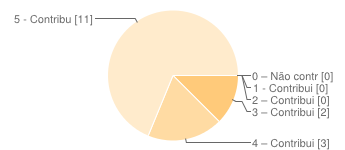
\includegraphics[width=.37\textwidth]{images/chart1.png}
  \end{center}
  \caption{Respostas do nível de contribuição do projeto na sua formação}
  \label{fig:core_concurrent}
\end{figure} 

A terceira questão trata, também em uma escala de 0 a 5, do quanto o projeto atrapalha de sua performance nas disciplinas da graduação. 19\% dos entrevistados responderam "3 - Atrapalha minha graduação da mesma forma que um estágio", 50\% dos entrevistados responderam "2 - Atrapalha moderadamente", 19\% dos entrevistados responderam "1 - Atrapalha pouco, menos que um estágio" e 13\% dos entrevistados responderam "0  Não atrapalha em nada na minha graduação".

\begin{figure}[htpb]
  \begin{center}
    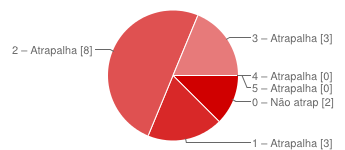
\includegraphics[width=.37\textwidth]{images/chart2.png}
  \end{center}
  \caption{Respostas do nível de performance nas disciplinas de graduação}
  \label{fig:core_concurrent}
\end{figure} 

A quarta questão averigua o quanto os conhecimentos adiquiridos durante a execução do projeto ajuda os entrevistados nas disciplinas da graduação, em uma escala de 0 a 5. 7\% dos entrevistados responderam "5 - Ajuda muito, sempre utilizo os conhecimentos adiquiridos nas disciplinas da graduação	", 47\% respondeu "4  Ajuda muito, utilizo os conhecimentos com frequência nas disciplinas da graduação", 27\% respondeu "3 - Ajuda, utilizo os conhecimentos nas disciplinas da graduação" 13\% respondeu "2 - Ajuda moderadamente, as vezes utilizo os conhecimentos adquiridos no projeto" e 7\% respondeu "1 – Ajuda um pouco, utilizo pouco os conhecimentos do projeto"

\begin{figure}[htpb]
  \begin{center}
    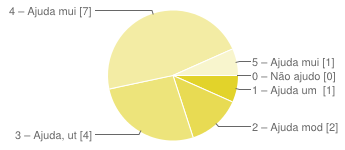
\includegraphics[width=.37\textwidth]{images/chart3.png}
  \end{center}
  \caption{Respostas do nível de conhecimento adquirido}
  \label{fig:core_concurrent}
\end{figure} 

E a quinta e última questão perguntou o quanto o entrevistado acredita que o projeto NSPB vai lhe dar de experiência para o mercado de trabalho, ainda em uma escala de 0 a 5. 38\% respondeu "5  O projeto me tornará experiente para o mercado de trabalho", 38\% respondeu "4 - O projeto me dará muita experiência para o mercado de trabalho" e 25\% respondeu "3 - O projeto me dará uma boa experiência para o mercado de trabalho".

\begin{figure}[htpb]
  \begin{center}
    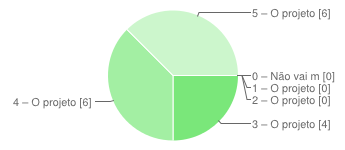
\includegraphics[width=.37\textwidth]{images/chart4.png}
  \end{center}
  \caption{Respostas do nível de experiência para o mercado de trabalho}
  \label{fig:core_concurrent}
\end{figure} 

%-------------------------------------------------------------------------------

\bibliographystyle{IEEEtran}
\bibliography{myReferences}
\end{document}
